\chapter{2020年\textsf{HDU} 概率论与数理统计期中练习题}

\begin{minipage}{0.32\textwidth}
    \textbf{开课学院}：理学院
      
    \textbf{课程编码}：A0714040
\end{minipage}
\hfill
\begin{minipage}{0.32\textwidth}
    \textbf{解析制作}：\textsc{Ljl, Zzr, Zwx, Xxy}

    \textbf{\,\hologo{TeX}~排版}：\textsc{Mingyu Hsia}
\end{minipage}
\hfill
\begin{minipage}{0.15\textwidth}
    \centering
    \begin{tikzpicture}
        \node [inner sep=0] at (0,0) {
            \qrcode[height=3em,level=M]{https://qm.qq.com/q/OlkSiy9W04}};
        \fill [color=white,rounded corners] (-.5em,-.5em) rectangle (.5em,.5em);
        \node [inner sep=0] at (0,0) {\color{MidnightBlue}\scriptsize\faIcon{qq}};
    \end{tikzpicture}

    \scriptsize\href{https://qm.qq.com/q/OlkSiy9W04}{\itshape 未央数学营}
\end{minipage}
\hfill
\begin{minipage}{0.15\textwidth}
    \centering
    \begin{tikzpicture}
        \node [inner sep=0] at (0,0) {
            \qrcode[height=3em,level=M]{http://weixin.qq.com/r/DBIABcHEqgnWKIVmb0eI}};
        \fill [color=white,rounded corners] (-.5em,-.5em) rectangle (.5em,.5em);
        \node [inner sep=0] at (0,0) {\color{DarkGreen}\scriptsize\faIcon{weixin}};
    \end{tikzpicture}

    \scriptsize\href{http://weixin.qq.com/r/DBIABcHEqgnWKIVmb0eI}{\itshape 未央学社}
\end{minipage}

\section{选择题}

\begin{problem}
    已知$A$、$B$、$C$为三个随机事件，则$A$、$B$、$C$都发生的事件为
    \begin{tasks}(4)
        \task $\overline{ABC}$
        \task $\overline A~\overline B~\overline C$
        \task $A\cup B\cup C$
        \task[\true] $ABC$
    \end{tasks}
\end{problem}
\solute2
\begin{solution}
    $A$、$B$、$C$都发生，则为$A\cap B\cap C$，用`$\cap$'表示.
\end{solution}

\begin{problem}
    设$A$、$B$是两个随机事件，则不能用$\overline{AB}$表示的事件是
    \begin{tasks}(2)
        \task[\true] $A$、$B$都不发生
        \task $A$、$B$不同时发生
        \task $A$、$B$中至多一个发生
        \task $A$、$B$中至少一个不发生
    \end{tasks}
\end{problem}
\solute2
\begin{solution}
    $\overline{AB}=\overline A\cap\overline B$. 所以A选项正确.
\end{solution}

\begin{problem}
    设$\overline A$与$B$为互相独立的两事件，且$P(\overline A)=0.7$，$P(B)=0.4$，则$P(AB)$的值为
    \begin{tasks}(4)
        \task $0.28$
        \task $0.7$
        \task[\true] $0.12$
        \task $0.4$
    \end{tasks}
\end{problem}
\solute2
\begin{solution}
    $P(A)=1-P(\overline A)=0.3$，$P(\overline AB)=0.28$，$P(AB)=P(B)-P(\overline AB)=0.12$.
\end{solution}

\begin{paracol}{2}
\begin{problem}
    离散型随机变量$X$的分布律如右图所示. 其分布函数为$F(x)$，且$F(2.2)=0.8$，则$a$的值为
    \begin{tasks}(4)
        \task $0.2$
        \task[\true] $0.5$
        \task $0.8$
        \task $0.4$
    \end{tasks}
\switchcolumn\vspace*{\fill}\centering
    \begin{tabular}{cccc}
        \toprule
        $X$ & $0$ & $2$ & $4$\\
        \midrule
        $P$ & $a$ & $0.3$ & $b$\\
        \bottomrule
    \end{tabular}\vspace*{\fill}
\end{problem}
\end{paracol}
\solute3
\begin{solution}
    $F(2.2)=a+0.3=0.8$，$a=0.5$.
\end{solution}

\begin{problem}
    设随机变量$X$和$Y$相互独立，且他们的分布函数分别为$F_X(x)$和$F_Y(y)$，则$Z=\min\{X,Y\}$的分布函数$F_Z(z)$是
    \begin{tasks}(2)
        \task $\min\{F_X(z),F_Y(z)\}$
        \task $F_X(z)F_Y(z)$
        \task $1-F_X(z)F_Y(z)$
        \task[\true] $1-[1-F_X(z)][1-F_Y(z)]$
    \end{tasks}
\end{problem}
\solute3
\begin{solution}
    $Z=\min\{X,Y\}$的分布函数$F_Z(z)$为
    \[\begin{aligned}[t]
        F_Z(z)&=F_{\min(X,Y)}(Z)=P\{Z\leq z\}=P\{\min(X,Y)\leq z\}=1-D\{\min(X,Y)>z\}\\&=1-P\{X>z\}P\{Y>z\}=1-[1-P(X\leq z)][1-P\{Y\leq z\}]
    \end{aligned}\]
\end{solution}

\begin{problem}
    设随机事件$A$表示``产品甲畅销，产品乙滞销''，则$A$的对立事件$\overline A$为
    \begin{tasks}(2)
        \task 产品甲滞销，产品乙畅销
        \task 产品甲、乙均畅销
        \task[\true] 产品甲滞销或产品乙畅销
        \task 产品甲畅销或产品乙滞销
    \end{tasks}
\end{problem}
\solute2
\begin{solution}\leavevmode\newline
    $A=\text{``甲畅销''}\cap\text{``乙畅销''}$，$\overline A=\text{``甲畅销''}\cap\text{``乙滞销''}=\overline{\text{``甲畅销''}}\cup\overline{\text{``乙滞销''}}=\text{``甲滞销''}\cup\text{``乙畅销''}$.
\end{solution}

\begin{problem}
    对于任意事件$A$、$B$，下列等式一定成立的是
    \begin{tasks}(2)
        \task $P(A|B)=P(A)$
        \task $P(AB)=P(A)P(B)$
        \task[\true] $P(A\overline B)=P(A)-P(AB)$
        \task $P(A\cup B)=P(A)+P(B)$
    \end{tasks}
\end{problem}
\solute2
\begin{solution}
    A、B、D的要求都为独立. C. $P(A\overline B)=P(A)-P(AB)$都成立.
\end{solution}

\begin{problem}
    设函数$f_X(x)$为某一随机变量$X$的概率密度函数，下列说法一定正确的是
    \begin{tasks}(2)
        \task $f_X(x)$的定义域为$[0,1]$
        \task[\true] $f_X(x)$的值域为$[0,1]$
        \task $f_X(x)$不恒等于$0$
        \task $f_X(x)$在$(-\infty,+\infty)$内连续
    \end{tasks}
\end{problem}
\solute2
\begin{solution}\leavevmode
    \begin{tasks}
        \task 均匀分布中$f_Z(x)$的定义域为$[a,b]$不一定为$[0,1]$.
        \task 均匀分布中令$b-a=1/2$，则$1/(b-a)=2$，$f_X(x)=2$不成立.\addtocounter{task}{1}
        \task 均匀分布中显然不连续.
    \end{tasks}
\end{solution}

\section{填空题}

\begin{problem}
    设$P(A)=0.4$，$P(B)=0.3$，$P(A\cup B)=0.5$，求$P(AB)$=\ans{$0.2$}.
\end{problem}
\begin{solution}
    由$P(A\cup B)=P(A)+P(B)-P(AB)$得$P(AB)=P(A)+P(B)-P(A\cup B)=0.2$.
\end{solution}

\begin{problem}
    10万把钥匙中有3把能打开一个门锁，现在任取两把，则能打开门锁的概率为\ans{$8/15$}.
\end{problem}
\begin{solution}
    无法打开门锁的概率为$C_7^2/C_{10}^2=7/15$，则能打开门锁的概率为$1-7/15=8/15$.
\end{solution}

\begin{problem}
    设随机变量$X\sim U(-1,7)$,则关于$y$的一元二次方程$y^2+Xy+1=0$有实根的概率为\ans{$5/8$}.
\end{problem}
\begin{solution}
    解有实根则$\Delta=X^2-4\geq0$，$X\leq-2$或$X\geq2$. 由于$X$满足均匀分布，故$P=5/8$.
\end{solution}

\begin{problem}
    已知随机变量$X\sim N(\mu,\sigma^2),P\{\mu<X<5\}=P\{1<X<\mu\}$，则$\mu=$\ans{$3$}.
\end{problem}
\begin{solution}
    由于$X$服从正态分布，两概率相等，说明区间关于$X=\mu$对称，故$\mu=(1+5)/2=3$.
\end{solution}

\begin{problem}
    设随机变量$X\sim\pi(\lambda)$，且$P(X=0)=e^{-2}$，则$\lambda=$\ans{$-2$}.
\end{problem}
\begin{solution}
    $X$满足泊松分布，则$P\{X=k\}=\e^{-\lambda}\lambda^k/k!$. 又$P(X=0)=\e^{-2}$，则$\e^{-\lambda}\lambda^0/0!=\e^{-2}$. 所以$\lambda=-2$.
\end{solution}

\begin{problem}
    设随机变量$X\sim U(-4,4)$，则关于$y$ 的一元二次方程$4y^2+4Xy+X+2=0$有实根的概率为\ans{$5/8$}.
\end{problem}
\begin{solution}
    由$\Delta=(4X)^2-16(X+2)\geq0$得$X\leq-1$或$X\geq2$. 由于$X$满足均匀分布，所以$P=(-1+4)+(4-2)/8=5/8$.
\end{solution}

\begin{problem}
    设随机变量$X$和$Y$相互独立，且分布律如下
    \begin{table}[htbp]
        \begin{minipage}[c]{.48\textwidth}
            \centering
            \begin{tabular}{ccccc}
                \toprule
                $X$ & $0$ & $1$ & $2$ & $3$\\
                \midrule
                $P$ & $1/2$ & $1/4$ & $1/8$ & $1/8$\\
                \bottomrule
            \end{tabular}
        \end{minipage}
        \hfill
        \begin{minipage}[c]{.48\textwidth}
            \centering
            \begin{tabular}{cccc}
                \toprule
                $Y$ & $-1$ & $0$ & $1$\\
                \midrule
                $P$ & $1/3$ & $1/3$ & $1/3$\\
                \bottomrule
            \end{tabular}
        \end{minipage}
    \end{table}

    则概率$P\{X+Y=2\}=$\ans{$1/6$}.
\end{problem}
\begin{solution}\leavevmode
    \begin{itemize}
        \item $X+Y=2$的情况分别有$(X=1,\ Y=1)$，$(X=2,\ Y=0)$，$(X=3,\ Y=-1)$.
        \item 由于$X$，$Y$满足独立分布，则有$P(X=a,\ Y=b)=P(X=a)\times(Y=b)$.
        \item $P\{X+Y=2\}=\frac14\times\frac13+\frac18\times\frac13+\frac18\times\frac13=\frac16$.
    \end{itemize}
\end{solution}

\clearpage
\section{计算题}

\begin{problem}
    已知$P(A)=1/4$，$P(B|A)=1/3$，$P(A|B)=1/2$. 求$P(A\cup B)$.
\end{problem}
\solute0
\begin{solution}
    \[\begin{aligned}
        P(A\cup B)&=P(A)+P(B)-P(AB)=P(A)+P(AB)/P(A|B)-P(AB)\\
        &=P(A)+\frac{P(A)P(B|A)}{P(A|B)}-P(A)P(B|A)=\frac13
    \end{aligned}\]
\end{solution}

\begin{paracol}{2}
\begin{problem}
    设离散型随机变量$X$数的分布函数为
    \[F(x)=\begin{cases}
        0, & x<2\\
        0.2, & -2\leq x<0\\
        0.6, & 0\leq x<3\\
        1, & x\geq3
    \end{cases}\]
    \switchcolumn
    \begin{enumerate}
        \item 求$X$的概率分布律.
        \item 求$Y=(X-1)^2$的概率分布律.
    \end{enumerate}
\end{problem}
\end{paracol}
\solute0
\begin{solution}
    $X$、$Y=(X-1)^2$的概率分布律如下. $Y$的可能取值为$1$，$4$，$9$.
    \begin{table}[htbp]
        \begin{minipage}{.48\textwidth}
            \centering
            \begin{tabular}{cccc}
                \toprule
                $X$ & $-2$ & $0$ & $3$\\
                \midrule
                $P(X=k)$ & $0.2$ & $0.4$ & $0.4$\\
                \bottomrule
            \end{tabular}
        \end{minipage}
        \hfill
        \begin{minipage}{.48\textwidth}
            \centering
            \begin{tabular}{cccc}
                \toprule
                $Y$ & $1$ & $4$ & $9$\\
                \midrule
                $P(Y=k)$ & $0.4$ & $0.4$ & $0.2$\\
                \bottomrule
            \end{tabular}
        \end{minipage}
    \end{table}
\end{solution}

\begin{problem}
    设随机变量$X$的概率密度为
    \[f(x)=\begin{cases}
        k\e^x, & x<0\\
        1/4, & 0\leq x\leq2\\
        0, & \text{else}
    \end{cases}\]
    \begin{tasks}[label=\arabic*.](3)
        \task 确定常数$k$.
        \task 求$X$的分布函数.
        \task 求$P\{1/2<X<3/2\}$.
    \end{tasks}
\end{problem}
\solute2
\begin{solution}\leavevmode
    \begin{enumerate}
        \item $\int_{-\infty}^{+\infty}f(x)\d x=\int_1^2k(1-1/x^2)\d x=1$，$k=2$.
        \item $x<1$时，$F(x)=0$；$x>2$时，$F(x)=1$；$x\in[1,2]$时，$F(x)=\int_1^xf(x)\d x=2(x-1)^2/x$.
        \[F(x)=\begin{cases}
            0, & x\in (-\infty,1)\\
            2(x-1)^2/x, & x\in[1,2]\\
            1, & x\in(2,+\infty)
        \end{cases}\]
        \item $P\{1/2<x<3/2\}=F(3/2)-F(1/2)=1/3$.
    \end{enumerate}
\end{solution}

\begin{problem}
    设随机变量$X$的概率密度为
    \[f(x)=\begin{cases}
        k(1-1/x^2), & 1\leq x\leq2\\
        0, & \text{else}
    \end{cases}\]
    \begin{tasks}[label=\arabic*.](3)
        \task 确定常数$k$.
        \task 求$X$的分布函数.
        \task 求$P\{1/2<X<3/2\}$.
    \end{tasks}
\end{problem}
\solute0
\begin{solution}\leavevmode
    \begin{enumerate}
        \item 根据连续型随机变量PDF规范性可知
        \[\int_{-\infty}^{+\infty}f(x)\d x=\int_{-\infty}^0k\e^x\d x+\int_0^2\frac14\d x+\int_2^{+\infty}0\d x=k+\frac12=1,\ k=\frac12\]
        \item 
        \begin{itemize}
            \item 当$x>2$时，$F(x)=\int_{-\infty}^xf(x)\d x=\int_{-\infty}^2f(x)\d x+\int_2^xf(x)\d x=1$.
            \item 当$x<0$时，$F(x)=\int_{-\infty}^xf(x)\d x=\int_{-\infty}^xk\e^x=\frac12\e^x$.
            \item 当$x\in[0,2]$时，$F(x)=\int_{-\infty}^0f(x)\d x+\int_0^xf(x)\d x=\int_{-\infty}^0\frac12\e^x\d x+\int_0^x\frac14\d x=\frac12+\frac14x$.
            \item 综上所述，$X$的分布函数为
            \[F(x)=\begin{cases}
                \frac12\e^x, & x<0\\
                \frac12+\frac14x, & 0\leq x\leq2\\
                1, & x>2
            \end{cases}\]
        \end{itemize}
        \item $P\{1<x<2\}=F(2)-F(3)=1-3/4=1/4$.
    \end{enumerate}
\end{solution}

\begin{paracol}{2}
\begin{problem}
    随机变量$(X,Y)$的概率分布律如右图所示.
    \begin{tasks}[label=\arabic*.](2)
        \task! 求关于$X$的边缘分布律.
        \task 求关于$XY$的分布律.
        \task 求$P\{X\leq1|Y=0\}$.
        \task! 判断$X$和$Y$是否相互独立，并说明理由.
    \end{tasks}
    \switchcolumn\vspace*{\fill}\centering
        \begin{tabular}{ccccc}
            \toprule
            \diagbox{Y}{X} & $-1$ & $0$ & $1$ & $2$\\
            \midrule
            $0$ & $0.1$ & $0.1$ & $0.2$ & $0.1$\\
            $1$ & $0.2$ & $0.1$ & $0.1$ & $0.1$\\
            \bottomrule
        \end{tabular}\vspace*{\fill}
\end{problem}
\end{paracol}
\solute0
\begin{solution}
    $X$的边缘分布律、$XY$的分布律分别为
    \begin{table}[H]
        \begin{minipage}{.42\textwidth}
            \centering
            \begin{tabular}{ccccc}
                \toprule
                $X$ & $-1$ & $0$ & $1$ & $2$\\
                \midrule
                $P$ & $0.3$ & $0.2$ & $0.3$ & $0.2$\\
                \bottomrule
            \end{tabular}
        \end{minipage}
        \hfill
        \begin{minipage}{.54\textwidth}
            \centering
            \begin{tabular}{ccccc}
                \toprule
                $XY$ & $0$ & $-1$ & $1$ & $2$\\
                \midrule
                $P$ & $0.6$ & $0.2$ & $0.1$ & $0.1$\\
                \bottomrule
            \end{tabular}
        \end{minipage}
    \end{table}
    \begin{itemize}
        \item $P\{X\leq1|Y=0\}=P\{x\leq1,Y=0\}/P\{Y=0\}=0.4/0.5=4/5$.
        \item 
        \begin{itemize}
            \item 由题意，当且仅当$X=1$，$Y=1$时$XY=1$.
            \item 而$P(X=1)P(Y=1)=0.3\times0.5\neq P(XY=1)=0.1$，所以不相互独立.
        \end{itemize}
    \end{itemize}
\end{solution}

\columnratio{.5}
\begin{paracol}{2}
\begin{problem}
    随机变量$(X,Y)$的密度函数为
    \[f(x,y)=\begin{cases}
        \e^{-y}, & 0\leq x\leq1,y>0\\
        0, & \text{else}
    \end{cases}\]
    \switchcolumn
    \begin{enumerate}
        \item 求$X$和$Y$边缘概率密度$f_X(x)$，$f_Y(y)$.
        \item 判断$X$与$Y$相互独立，并说明理由.
        \item 求$Z=Y/X$的概率密度函数$f_Z(x)$.
    \end{enumerate}
\end{problem}
\end{paracol}
\solute2
\begin{solution}\leavevmode
    \begin{enumerate}
        \item 
        \begin{itemize}
            \item $f_X(x)=\int_{-\infty}^{+\infty}f(xy)\d y=\int_0^{+\infty}\e^{-y}\d y=1$，$0\leq x\leq1$.
            \item $f_Y(x)=\int_{-\infty}^{+\infty}f(xy)\d x=\int_0^1\e^{-y}\d x=-\e^{-y}$，$y>0$.
        \end{itemize}
        \[f_X(x)=\begin{cases}
            1, & x\in[0,1]\\0, & \text{else}
        \end{cases},\ f_Y(y)=\begin{cases}
            \e^{-y}, & y\in(0,+\infty)\\0, & \text{else}
        \end{cases}\]
        \item 当$0\leq x\leq1$，$y>0$时，$f(x,y)=f_X(x)\cdot f_Y(y)$，所以二者相互独立.
        \item $z>0$时，$f_{Y/X}(z)=\int_{-\infty}^{+\infty}\abs{x}f(x,xz)\d x=\int_0^1\abs{x}\e^{-xz}\d x=(-z+\e^z)\e^{-z}/z^2$. 所以
        \[f_Z(z)=\begin{cases}
            (-z+\e^z-1)\e^{-z}/z^2, & z\in(0,+\infty)\\
            0, & \text{else}
        \end{cases}\]
    \end{enumerate}
\end{solution}

\begin{problem}
    市场上出售的某种商品由三个厂家同时供货，其供应量第一厂家为第二厂家的两倍，第二、第三厂家相等，且第一、第二、第三厂家的次品率依次为2\%，2\%，4\%。若在市场上随机购买一件商品为次品，问该件商品是第一厂家生产的概率为多少？
\end{problem}
\solute1
\begin{solution}
    $X$表示是否次品，$x=1$为次品，$Y$表示上架.
    \[P(y=1|x=1)=\frac{P(y\leq1)P(x=1|y=1)}{P(x=1)}=\frac{50\%\times2\%}{50\%\times2\%+25\%\times2\%+25\%\times4\%}=2/5\]
\end{solution}

\begin{problem}
    设连续型随机变量$X$与$Y$相互独立，且具有概率密度分别为
    \[f_X(x)=\begin{cases}
        2\e^{-2x}, & x>0\\
        0, & \text{else}
    \end{cases},\ 
    f_Y(x)=\begin{cases}
        \e^{-y}, & y>0\\
        0, & \text{else}
    \end{cases}\]
    求$P(Y\leq1|X=1)$.
\end{problem}
\begin{solution}
    $P(y\leq1|x=1)=P(y_1\leq1)=\int_{-\infty}^1f_Y(y)\d y=\int_0^1\e^{-y}\d y=-\e^{-y}\big|_0^1=1-\e^{-1}$.
\end{solution}

\begin{problem}
    已知5\%的男性和25\%的女性是色盲，假设男性女性各占一半。现随机地挑选一人，利用全概率公式求此人恰好是色盲者的概率.
\end{problem}
\solute1
\begin{solution}
    由全概率公式$5\%\times50\%+25\%\times50\%=15\%$.
\end{solution}

\begin{paracol}{2}
\begin{problem}
    随机变量$(X,Y)$的密度函数为
    \[f(x,y)=\begin{cases}
        \e^{-(x+y)}, & 0\leq x\leq1,y>0\\
        0, & \text{else}
    \end{cases}\]
    \switchcolumn
    \begin{enumerate}
        \item 求$X$和$Y$的边缘概率密度$f_X(x)$，$f_Y(y)$.
        \item 判断$X$、$Y$相互独立，并说明理由.
        \item 求$Z=(Y-X)/2$的概率密度函数$f_Z(z)$.
    \end{enumerate}
\end{problem}
\end{paracol}
\solute3
\columnratio{.64}
\begin{solution}\leavevmode
    \begin{enumerate}
        \item $f_X(x)=\begin{cases}
            0, & x<0\ \text{or}\ x>1\\
            \int_{-\infty}^{+\infty}\e^{-y}\d y=1, & 0\leq x\leq1
        \end{cases}$，
        $f_Y(x)=\begin{cases}
            0, & y\leq0\\
            \e^{-y}, & y>0
        \end{cases}$
        \item $f_X(x)f_Y(y)=f(x,y)$，所以$X$与$Y$相互独立.
        \item 考察$F_Z(z)=[P(Y-X)/{2}\leq Z]$
        \begin{itemize}
            \item 当$z<-0.5$时，$F_Z(z)=0$
            \item 当$-0.5<z\leq0$时，$F_Z(z)=\int_{-2z}^1\d x\int_0^{x+2z}f(x,y)\d y=2z+\e^{-2z-1}$.
            \item 当$z>0$时，$F_Z(z)=\int_0^1\d x\int_{2z}^{1+2z}\e^{-y}\d y=(1-\e^{-1})\e^{-2z}$. 所以$Z$的概率密度函数为
        \end{itemize}
        \[f_Z(z)=F'_Z(z)=\begin{cases}
            0, & z\leq-0.5\\
            2-2\e^{-2z}, & -0.5<z\leq0\\
            -2(1-\e^{-1})\e^{-2z}, & z>0
        \end{cases}\]
    \end{enumerate}
\end{solution}

\begin{problem}\leavevmode
    \begin{enumerate}
        \item 证明：事件$A$、$B$相互独立的充分必要条件是$P(A|B)=P(A|\overline B)$.
        \item 已知$P(A)=0.9$，$P(B)=0.8$. 试证：$P(A|B)\geq0.875$.
    \end{enumerate}
\end{problem}
\solute{5}
\begin{solution}
\begin{proof}\leavevmode
    \begin{enumerate}
        \item $P(A|B)=P(AB)/P(B)$，$P(A|\overline B)=P(A\overline B)/P(\overline B)$.
        \begin{itemize}
            \item 若$A$、$B$独立，则$P(AB)=P(A)P(B)$，$P(A\overline B)=P(A)P(\overline B)$. 显然$P(A|B)=P(A|\overline B)$.
            \item 若$P(A|B)=P(A|\overline B)$，则$P(AB)/P(B)=P(A\overline B)/P(\overline B)=[P(A)-P(AB)]/[1-P(B)]$.
        \end{itemize}

        \begin{paracol}{2}
            即得$P(AB)=P(A)P(B)$，$A$、$B$独立.\qed
            \item
            \begin{itemize}
                \item $P(A|B)=P(AB)/P(B)$.
                \item 令$P(AB)=t$，$P(\overline A~\overline B)=t-0.7\geq0$，得$t\geq0.7$.
                \item 所以$P(A|B)\geq0.7/0.8=0.875$.\qed
            \end{itemize}
            \switchcolumn\centering
                \begin{tabular}{cccc}
                    \toprule
                    & $A$ & $\overline A$ & $\Omega$\\
                    \midrule
                    $B$ & $t$ & $0.8-t$ & $0.3$\\
                    $\overline B$ & $0.9-t$ & \\
                    $\Omega$ & $0.9$\\
                    \bottomrule
                \end{tabular}
        \end{paracol}
    \end{enumerate}
    \renewcommand\qedsymbol{}
\end{proof}
\end{solution}